\documentclass[letterpaper]{article}

% To use numbered citations instead, uncomment the following line:
% \PassOptionsToPackage{numbers,compress}{natbib}
% Keep rl_project.sty in the same folder as this file.
\usepackage[final]{rl_project}

\usepackage[utf8]{inputenc}
\usepackage[T1]{fontenc}
\usepackage{hyperref}
\usepackage{url}
\usepackage{booktabs}
\usepackage{amsfonts}
\usepackage{nicefrac}
\usepackage{microtype}
\usepackage{graphicx}

\title{Formatting Example (RL Project)}

% Replace the example authors with all members of your group.
\author{
  Joshua~B.~Evans \qquad Sophia~Jones \\
  Department of Computer Science \\
  University of Bath \\
  Bath, BA2 7AY \\
  \texttt{\{jbe25,sj2073\}@bath.ac.uk}
}

\begin{document}

\maketitle

\section{Using the Template}

This document illustrates how to format text, headings, citations, figures, tables, and references using the supplied report template. It is a \emph{formatting example}, not an example of a completed coursework report. Follow the assessment specification and the separate blank report template for the required structure and content.

To get started, put \verb|rl_project.sty| in the same folder as your \verb|.tex| file, and keep \verb|\usepackage[final]{rl_project}| in the preamble (before \verb|\begin{document}|). The style file controls the page layout and other formatting. Use the blank template for your submission, replacing the example title and authors with your group's details.

Your report's main body should respect the page limit outlined in the coursework specification. The specified page limit \emph{includes} figures, tables, and their captions. The Generative AI Use Declaration, References, and Appendices are excluded from this limit. Essential material should appear in the main body; appendices are for supporting details.

Do not include a separate title page or table of contents. Your report should begin with the \emph{Problem Definition} section immediately after the title and author information on the first page.

\section{Headings}

Use \verb|\section| for the main report sections specified in the assessment, including \emph{Problem Definition}, \emph{Background}, \emph{Method}, and \emph{Results}. The style file handles the appearance of headings automatically.

\subsection{Second-level headings}

Use \verb|\subsection| to divide a section into smaller topics.

\subsubsection{Third-level headings}

Use \verb|\subsubsection| where further subdivision is useful.

\paragraph{Paragraph headings.}

The \verb|\paragraph| command produces an inline, bold heading, as demonstrated here.

Use the \verb|\subsection| and \verb|\subsubsection| commands sparingly. Each heading takes up valuable vertical space, and excessive subdivision can quickly eat into your page limit.

\section{Citations and References}

The \verb|rl_project| style loads \verb|natbib| by default. You can cite a source as part of a sentence using \verb|\citet|, as in \citet{hasselmo1995}, or use \verb|\citep| for a parenthetical citation \citep{alexander1995}. These references are retained solely as formatting examples; cite literature relevant to your own project, including methods and ideas introduced in lectures.

You may use any appropriate referencing style, provided you apply it consistently. We recommend managing references using a separate \verb|.bib| file, as this makes them easier to organise and maintain. For guidance, see \href{https://www.overleaf.com/learn/latex/Bibliography_management_with_natbib}{Overleaf's guide to bibliography management with natbib}. This example instead uses the \verb|thebibliography| environment to keep it self-contained, but this approach is not generally recommended.

\section{Figures}

Figure~\ref{fig:example} illustrates figure placement, captioning, and cross-references. The box is a placeholder rather than an experimental result. To include your own image, replace the placeholder with \verb|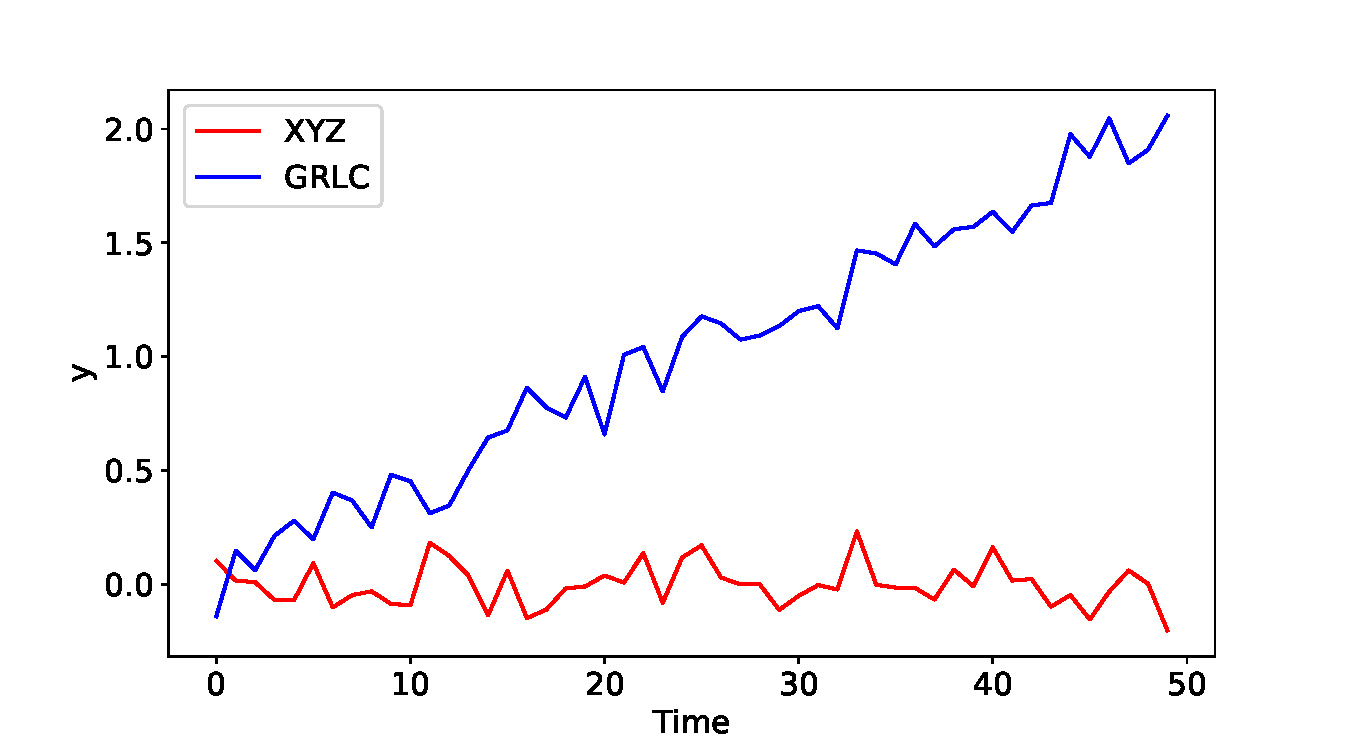
\includegraphics[width=0.7\textwidth]{some_figure.pdf}| and upload that file to your project.

\begin{figure}[htbp]
  \centering
  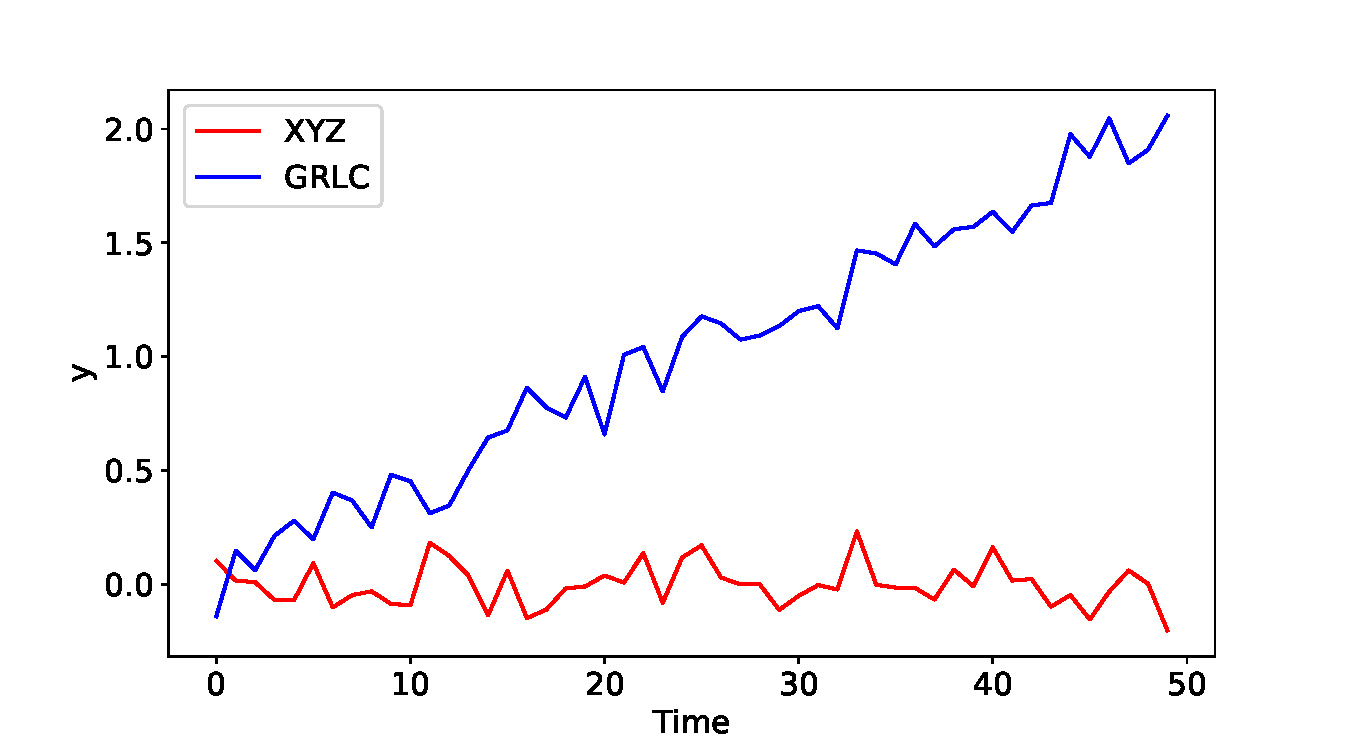
\includegraphics[width=0.7\textwidth]{some_figure.pdf}
  \caption{Example figure caption.}
  \label{fig:example}
\end{figure}

Place the caption below a figure, assign it a \verb|\label|, and refer to it using \verb|\ref| elsewhere in the report rather than typing its figure number manually. Ensure that labels, legends, and plotted lines remain legible, including when printed in greyscale.

\section{Tables}

You may wish to present some of your experimental results using tables. Table~\ref{tab:example} demonstrates table formatting using the \verb|booktabs| package.

\begin{table}[htbp]
  \caption{Example table caption.}
  \label{tab:example}
  \centering
  \begin{tabular}{lll}
    \toprule
    \multicolumn{2}{c}{Part}                   \\
    \cmidrule(r){1-2}
    Name     & Description     & Size ($\mu$m) \\
    \midrule
    Dendrite & Input terminal  & $\sim$100     \\
    Axon     & Output terminal & $\sim$10      \\
    Soma     & Cell body       & up to $10^6$  \\
    \bottomrule
  \end{tabular}
\end{table}

Place the caption above a table. As with figures, use \verb|\label| and \verb|\ref| to reference tables. In your report, tables should present information relevant to your methods or evaluation.

\section{Footnotes}

Use footnotes sparingly. If needed, LaTeX places them at the bottom of the page when you use \verb|\footnote|, as in this example\footnote{Example footnote.}.

\section{Collaborating}

You can access Overleaf Premium for free by linking your University of Bath email address to your Overleaf account. Overleaf allows you to edit LaTeX documents collaboratively in real time (much like you can edit WYSIWYG documents in Google Docs), and is the recommended way to work together on your group report.

\clearpage
\section*{Generative AI Use Declaration}

State whether your group used GenAI tools and, if so, how and to what extent.

\small
\begin{thebibliography}{9}

\bibitem[Alexander and Mozer(1995)]{alexander1995}
Alexander, J.~A. and Mozer, M.~C. (1995).
Template-based algorithms for connectionist rule extraction.
In G.~Tesauro, D.~S. Touretzky, and T.~K. Leen (eds.),
\textit{Advances in Neural Information Processing Systems 7}, pp.~609--616.

\bibitem[Bower and Beeman(1995)]{bower1995}
Bower, J.~M. and Beeman, D. (1995).
\textit{The Book of GENESIS: Exploring Realistic Neural Models with the GEneral NEural SImulation System}.
TELOS/Springer--Verlag.

\bibitem[Hasselmo et~al.(1995)]{hasselmo1995}
Hasselmo, M.~E., Schnell, E., and Barkai, E. (1995).
Dynamics of learning and recall at excitatory recurrent synapses and cholinergic modulation in rat hippocampal region CA3.
\textit{Journal of Neuroscience}, 15(7):5249--5262.

\end{thebibliography}
\normalsize

\clearpage
\section*{Appendices}

Appendices are intended for supplementary material that supports the main report, such as additional results, implementation details, or information needed to reproduce your experiments. Any figures, results, or explanations central to your investigation must appear in the main body of the report. Moving essential information to the appendices simply to save space is not acceptable and will result in lost marks.

Appendices are excluded from the page limit and should be referenced in the main report. Any appendices not referenced directly in the main body of the report will not be read.

\subsection*{Appendix A: Example Appendix}

Additional supporting material can be placed here.

\end{document}